\begin{figure}[t]
   \centering
   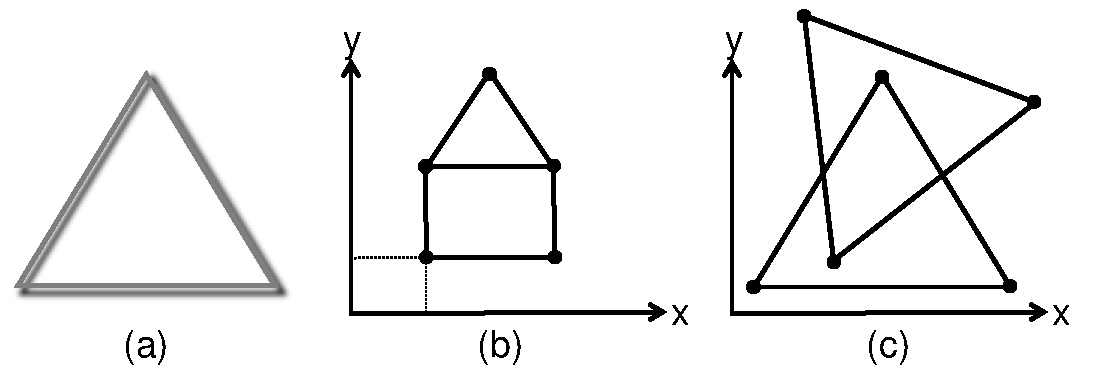
\includegraphics[width=\columnwidth]{CookieCAD.pdf}%
   \vspace{-1em}
   \caption{CookieCAD: (a) Real-life cookie cutter. (b) House-like 
shape with line-sharing. (c) Invalid shape (due to overlaps).}%  
   \label{fig:CookieCAD}
\end{figure}

\section{Case Study: CookieCAD}
\label{sec:CS}

\enlargethispage{6pt}


Computer-Aided Design (\textsc{cad}) \cite{B:Groover-Zimmers:2008} promotes the
use of computer systems to assist the creation, modification, analysis and
optimisation of a design.
A design may describe any physical, 3D object, e.g., engines or planes for
analysing heat and fluid transfers, bridges and wind mills to estimate the
dynamic response of the mechanical structure to various environmental
variations. \textsc{cad} is often paired with Computer-Aided Manufacturing
(\textsc{Cam}) to help plan, manage and control the operations around the
process of bringing 3D designs to life. Historically, techniques and tools
heavily rely on geometry, solid and surface mathematical formalisms. This
particular set of processes operated over a selected bunch of formalisms and
languages makes \textsc{cad} a paradigm on its own.

We propose to illustrate our formal framework with a simplified variant of 
\textsc{cad} named Cookie\textsc{cad} (\textsc{ccad}) that helps design simple 
cookie cutters, as illustrated in Fig.~\ref{fig:CookieCAD}(a). A cookie cutter 
adopts a simple shape (triangle, rectangle, star, etc.) represented by 2D geometric 
lines (noted $L$) which are specified based on the definition of two points in 
no particular order (noted $P$) placed in a cartesian plane (using x-/y- 
coordinates). In order to be manufacturable, points shall not be placed too 
close to each other (the exact distance tolerance depends on the machinery 
used), and shall represent closed polygons that may share some lines (as 
illustrated in Fig.~\ref{fig:CookieCAD}(b) for a house-like cutter, with the 
triangular roof placed over the rectangular base). Consequently, lines shall not 
cross each others as illustrated in Fig. \ref{fig:CookieCAD}(c), which results 
in an \emph{invalid} cookie cutter. At manufacturing time, such a design shall 
be associated with a width to build a 3D physical object: the precision of the 
machine may finally discard some of the designs presented on Fig. 
\ref{fig:CookieCAD}(a) if it is not able to cut or fold metal pieces that size.

\begin{figure}[t]
   \centering
   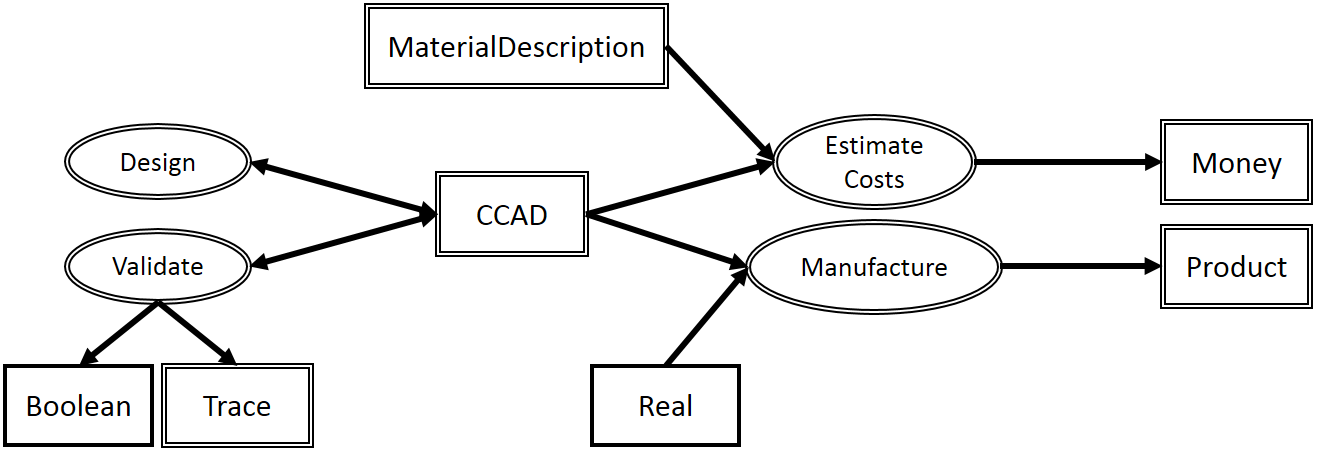
\includegraphics[width=0.98\columnwidth]{CCAD_FTG}
   \caption{$\mathsf{FTG_{CCAD}}$: an x\textsc{ftg} for \textsc{ccad} 
activities.}%
   \label{fig:CCAD-FTG}%
\end{figure}

Figure \ref{fig:CCAD-FTG} depicts a possible, simplified x\textsc{ftg} for 
\textsc{ccad} named $\mathsf{FTG_{CCAD}}$. It includes four transformations 
templates represented as double-rounded ellipses named $\mathsf{Design}$, 
$\mathsf{Validate}$, $\mathsf{EstimateCosts}$ and $\mathsf{Manufacture}$. As an 
example, a repository would have to retrieve a transformation corresponding to
the following signature: $\mathsf{Validate} \mapsto 
(\langle\mathsf{CCAD}\rangle, \langle \mathsf{CCAD}, \mathsf{Boolean}, 
\mathsf{Trace}\rangle, \top)$, meaning that $\mathsf{Validate}$ is automatic and 
takes as source a $\mathsf{CCAD}$ model and produces back the source 
$\mathsf{CCAD}$ (notice the double arrow from/to $\mathsf{CCAD}$), and a 
boolean value, indicating whether the source model is valid or not, in which 
case a $\mathsf{Trace}$ model is produced. The target $\mathsf{CCAD}$ model may 
be discarded by some tools, but nothing prevents a repository to select 
transformations that may additionnally decorate the target with information 
from the trace model to help \textsc{ccad} designers grasp their errors' 
origins more easily, or keep traces and models cleanly separated, since both 
behaviours match $\mathsf{Validate}$'s signature. All transformation and 
metamodel names in Fig.~\ref{fig:CCAD-FTG} are templates (meaning they belong 
to $\mathsf{TMMName}$ or $\mathsf{TTName}$) except $\mathsf{Boolean}$ and 
$\mathsf{Real}$, which is used as a source parameterising the width of the 
cookie cutter design in order to produce the physical 3D cutter.

\begin{figure}[t]
\centering

\includegraphics[width=0.98\columnwidth]{CCAD-MM}
\caption{Template metamodel $\mathsf{CCAD}$ in $\mathsf{FTG_{CCAD}}$ 
(cf. Fig. \ref{fig:CCAD-FTG}).}
\label{fig:CCAD-MM}%

\vspace{-0.5cm}
\end{figure}

These template transformations make a central use of the $\mathsf{CCAD}$ 
language that would handle the visual representation, design, validation, 
debugging, etc. of a cookie cutters designs, based on the template metamodel 
of Fig. \ref{fig:CCAD-MM}: a $\mathsf{CCAD}$ model is defined by a set 
of lines delimited by exactly two points, in no particular order, having real 
coordinates on a 2D plane. The semantics of such a metamodel captures all points 
in an Euclidian plane between any pair of points defining a line.
% , as captured 
% by the following semantic mapping (where $m = \frac{y'-y}{x'-x}$ and w.l.o.g. 
% $x' \geq x$).
% \begin{displaymath}
%    \begin{small}
%       \begin{array}{rcl}
%          \SMapping & \colon & \!\!\!
%             \begin{array}[t]{rcl}
%                \CCAD &\to& \wp(\wp(\mathbb{R}^2)) \\
%                    o &\mapsto& \lbrace \lbrace u,v\rbrace \;|\; \exists 
% u,v\in \mathbb{R}.\; 
%                     \forall x \leq u \leq x'. \\
% & & v{=}m{*}u{+}\left(y{-}m{*}x\right), o{=}\lbrace \lbrace x, y \rbrace, 
% \lbrace x', y' \rbrace \rbrace,
% %%
%             \end{array}\\
%       \end{array}
%    \end{small}
% \end{displaymath}




Fig.~\ref{fig:CCAD-PM-Full} depicts a candidate, well-formed \textsc{Pm}s 
named $\mathsf{PM_{Full}}$.
It arranges three transformations from $\mathsf{FTG_{CCAD}}$ in a sequential 
fashion: starting from scratch, a designer starts iteratively create a
design, then manufacture it once it has been validated. This workflow does not 
prohibit manufacturing of expensive designs, since $\mathsf{EstimateCosts}$ is 
left out.
Enforcing such a scenario requires specifying properties specifically targeting 
$\mathsf{PM_{Full}}$'s topology, asking at least $\mathsf{EstimateCosts}$'s 
presence in the \textsc{Pm} in order to break $\mathsf{PM_{Full}}$ 
well-formedness.
% \begin{wrapfigure}[11]{l}{0.1\textwidth}
%   \begin{center}
%     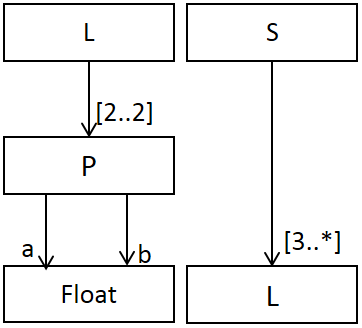
\includegraphics[width=0.1\textwidth]{CCAD_Props}
%   \end{center}
%   \caption{Pattern Properties for $\mbox{CAD}_1$ and $\mbox{CAD}_2$.}
%   \label{fig:PatternProperties}
% \end{wrapfigure}
%
Refering to Tab. \ref{tab:Properties}, $\mbox{CAD}_1$ and $\mbox{CAD}_2$ are 
easily recognised as property 
patterns over a metamodel manipulating \textsc{cad} designs; while 
$\mbox{CAD}_3$ specifies a property characterising the existence of a 
transformation that produces a final, real-life 3D product. Fig.~\ref{fig:CCAD-MM} 
shows possible patterns for capturing them in a 
\textsc{Mof}-like syntax. Assuming one has explicit languages 
for expressing the required properties, this would built a set of 
paradigmatic properties $\pi_{\mathsf{CAD}}\in\Pi$ that constitute part of 
our $\mathsf{CAD}$ paradigm (i.e. $\mathsf{CAD} \mapsto \pi_{\mathsf{CAD}}$ in 
the sense of Def. \ref{def:Paradigm}).


We have built a paradigmatic structure $\mathsf{PS_{CCAD}} = (MM, 
\{\mathsf{W_{CCAD}}\})\in\PS$ with only one workflow $\mathsf{W_{CCAD}} = 
(\mathsf{FTG_{CCAD}}, \mathsf{PM_{Full}})\in\mathbb{W}(TR, MM)$ relying on 
transformation $TR$ and metamodel names $MM$ as described in Fig. 
\ref{fig:CCAD-FTG}. \emph{Now, does $\mathsf{PS_{CCAD}}$ qualify as a 
$\mathsf{CAD}$ (simplified) paradigm?}

Properties $\mbox{CAD}_1$ and $\mbox{CAD}_2$ are easily checked on the 
$\mathsf{CCAD}$ metamodel by matching the classes from the template properties 
to their corresponding class (namely, $\mathsf{L}$ and $\mathsf{P}$ to 
$\mathsf{Line}$ and $\mathsf{Point}$, then references $\mathsf{}$ and 
$\mathsf{b}$ to $\mathsf{x}$ and $\mathsf{y}$, and finally $\mathsf{S}$ to 
$\mathsf{CCAD}$ itself). Property $\mbox{CAD}_2$ may be matched to the 
transformation template $\mathsf{Manufacture}$, with a template 
$\mathsf{Product}$ yet to be retrieved from the repository.  

% \begin{figure}[t]
% \centering 
% 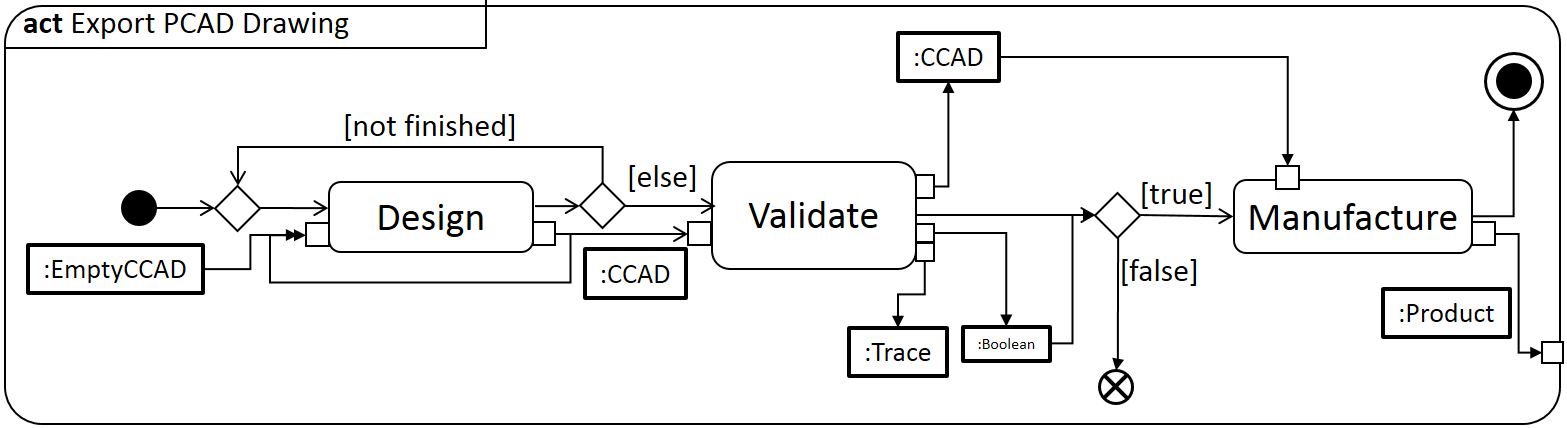
\includegraphics[width=0.98\columnwidth]{CCAD_PM}
% \caption{$\mathsf{PM_{Full}}$: a possible \textsc{Pm} manufacturing 
% \textsc{ccad} designs at the expanse of your company!} 
% \label{fig:CCAD-PM-Full}%
% \end{figure}

